% =================================================================
% This is an assignment report template (in LaTeX) for the following course:
% PHYS 421 Parallel Computing
% Instructors: Sergiy Bubin, Bekdaulet Shukirgaliyev
% Version: 2025.08.10
% =================================================================

\documentclass[11pt,a4paper]{article}

% ---------- Encoding, fonts, language ----------
\usepackage[T1]{fontenc}
\usepackage[utf8]{inputenc}
\usepackage{lmodern}
\usepackage[english]{babel}

% ---------- Geometry & spacing ----------
\usepackage[a4paper,margin=1in]{geometry}
\usepackage{setspace}
\onehalfspacing
\usepackage{parskip} % space between paragraphs, no indent

% ---------- Math & symbols ----------
\usepackage{amsmath,amssymb,amsthm}
\usepackage{siunitx}
\sisetup{detect-all=true}

% ---------- Tables & graphics ----------
\usepackage{graphicx}
\usepackage{booktabs}
\usepackage{xcolor}
\usepackage{float}
\usepackage{subcaption}
\usepackage{mwe} % provides example-image-a
\usepackage{hologo}

% ---------- Hyperlinks & clever references ----------
%\usepackage[hidelinks]{hyperref}
\usepackage[colorlinks=true,urlcolor=blue,bookmarks=true,citecolor=magenta,breaklinks=true,pdftex]{hyperref}
\usepackage[nameinlink,capitalise]{cleveref}

% ---------- Code listings (default: listings) ----------
\usepackage{listings}
\lstdefinestyle{pcstyle}{
	basicstyle=\ttfamily\footnotesize,  %change \footnotesize to \small if the font in code snippets appears too small for reading
	numberstyle=\tiny, numbers=left, numbersep=8pt,
	showstringspaces=false, showtabs=false, showspaces=false,
	breaklines=true, frame=single, rulecolor=\color{black!20},
	keywordstyle=\color{blue!90!black},
	commentstyle=\color{green!65!black},
	stringstyle=\color{orange!80!black},
	tabsize=2,
	captionpos=b
}
\lstset{style=pcstyle}

% ---------- Optional: minted for code (requires shell-escape) ----------
% To use minted on Overleaf: Menu -> Latex -> Enable shell escape.
% Then uncomment the two lines below and comment out the listings section above.
% \usepackage[outputdir=_minted,cache=false]{minted}
% \setminted{fontsize=\small,breaklines,frame=single}

% ---------- PGFPlots for plots ----------
\usepackage{gincltex}
\usepackage{pgfplots}
\pgfplotsset{compat=1.18}
\usepackage{pgfplotstable}
\usepgflibrary{plotmarks}
\usetikzlibrary{calc}
\usetikzlibrary{positioning,arrows.meta}

% ---------- Bibliography ----------
\usepackage[
backend=biber,
style=numeric-comp, % compress ranges like [1–3]
sorting=none,
sortcites=true      % sort inside each \cite{...}
]{biblatex}
\addbibresource{references.bib}

% ---------- Utilities ----------
\usepackage{etoolbox} % for \IfFileExists

% ---------- Custom metadata commands ----------
% Replace X with the actual assignment number
\newcommand{\assignmentnumber}{2}
% Insert actual report title
\newcommand{\assignmenttitle}{Monte Carlo Estimation of n-Dimensional $\ell^p$ Sphere Volumes}
% Insert your name
\newcommand{\studentname}{Adilet Akimshe}
% Replace XXXXXXXXX with your actual Student ID
\newcommand{\studentid}{202194337}
% Insert course code: PHYS 421, PHYS 521, or PHYS 721
\newcommand{\coursecode}{PHYS 421}  
% Insert course name: Parallel Computing or Parallel Programming for Scientific Computing
\newcommand{\coursename}{Parallel Computing} 

\newcommand{\honor}{I affirm that this work complies with Nazarbayev University academic integrity policies and the policies regarding the use of AI tools outlined in the course syllabus}

% ---------- Title ----------
\title{Assignment Report \#\assignmentnumber \\ \assignmenttitle}
\author{Student Name: \studentname \ (ID: \studentid) \\ Course: \coursecode \ \coursename
}
\date{Submitted: \today}

% =================================================================
\begin{document}
	\maketitle
	
	\begin{center}
		{Software packages used:} \\
		\begin{tabular}{|l|l|}
			\hline
			GCC 13.3.0               &  Main code compilation \\
			OpenMP                   &  Parallelization framework \\
			Python 3.12              &  Data analysis and plotting \\
			GNU Make                 &  Build automation \\
			\hline
		\end{tabular}
	\end{center}
	
	\begin{center}
		{AI tools used:} \\
		\begin{tabular}{|l|l|}
			\hline
			Claude 4 Sonnet         & Code development assistance, report writing \\
			\hline
		\end{tabular}
	\end{center}
	\vspace{2em}
	
	\begin{abstract}
		\noindent
		This report presents a parallel Monte Carlo implementation using OpenMP to estimate volumes of n-dimensional $\ell^p$ spheres. The method samples random points uniformly within hypercubes and counts those falling inside the p-sphere boundary. Experiments were conducted on a 4-core Intel i5-7200U system running Ubuntu 24.04 with GCC 13.3.0. Key results include: (1) Monte Carlo error scaling follows the theoretical $\mathcal{O}(1/\sqrt{N})$ relationship, achieving 0.063\% relative error with 6.4M samples; (2) parallel scaling shows good performance up to 2 threads with 2.28× speedup, but efficiency degrades beyond this due to system limitations; (3) validation against analytical formulas demonstrates excellent agreement with average relative error of 0.19\% across dimensions 2-10; (4) static scheduling generally outperforms dynamic scheduling for this embarrassingly parallel workload.
	\end{abstract}
	% =================================================================
	
	\section{Introduction and Problem Statement}
	
	Monte Carlo methods provide a powerful approach for estimating integrals and volumes in high-dimensional spaces where analytical solutions become computationally prohibitive. This assignment focuses on estimating the volume of n-dimensional spheres defined in the $\ell^p$ norm, which encompasses a rich family of geometric shapes from diamond-like ($p < 1$) to hypercube-approaching ($p \to \infty$) forms.
	
	The n-dimensional $\ell^p$ ball of radius $R$ is defined as the set of points satisfying:
	\begin{equation}\label{eq:p_ball_definition}
		|x_1|^p + |x_2|^p + \ldots + |x_n|^p \le R^p
	\end{equation}
	
	where $p > 0$ can take any positive real value. The exact analytical volume is given by:
	\begin{equation}\label{eq:exact_volume}
		V_n^p(R) = \frac{[2\Gamma(1+1/p)]^n}{\Gamma(1+n/p)} R^n
	\end{equation}
	
	where $\Gamma$ is the Euler gamma function.
	
	The primary objectives of this work are to: (1) implement both serial and parallel Monte Carlo volume estimation algorithms; (2) analyze accuracy scaling with sample size $N$; (3) evaluate parallel performance and efficiency across different thread counts; (4) validate results against analytical formulas; and (5) investigate the effects of OpenMP scheduling strategies.
	
	\section{Hardware and Software Environment}
	
	All experiments were conducted on a laptop system with the specifications listed in Table~\ref{table:system_specs}.
	
	\begin{table}[H]
		\centering
		\caption{System specifications and software environment.}
		\label{table:system_specs}
		\begin{tabular}{ll}
			\toprule
			Component & Specification \\
			\midrule
			CPU & Intel Core i5-7200U @ 2.50GHz \\
			Cores/Threads & 2 physical cores, 4 logical threads \\
			Memory & 8GB DDR4 \\
			OS & Ubuntu 24.04 LTS \\
			Compiler & GCC 13.3.0 \\
			OpenMP & Version included with GCC 13.3.0 \\
			Python & 3.12 (matplotlib, pandas, numpy) \\
			\bottomrule
		\end{tabular}
	\end{table}
	
	\section{Methods and Implementation}
	
	\subsection{Monte Carlo Algorithm}
	
	The Monte Carlo volume estimation algorithm embeds the n-dimensional $\ell^p$ ball within an axis-aligned hypercube of side length $2R$, giving a hypercube volume of $(2R)^n$. The algorithm generates $N$ uniformly distributed random points within this hypercube and counts the number of "hits" (points falling inside the p-sphere). The volume estimate is then:
	
	\begin{equation}\label{eq:monte_carlo_estimate}
		V_{est} = \frac{\text{hits}}{N} \times (2R)^n
	\end{equation}
	
	The standard error of Monte Carlo methods scales as $\mathcal{O}(1/\sqrt{N})$, providing a theoretical framework for accuracy analysis.
	
	\subsection{Parallel Implementation}
	
	The parallel implementation uses OpenMP to distribute the sampling loop across multiple threads. Key implementation details include:
	
	\begin{lstlisting}[language=C, caption={Core parallel sampling loop structure}, label={lst:parallel_core}]
		#pragma omp parallel
		{
			int thread_id = omp_get_thread_num();
			unsigned int thread_seed = seed + 1337 * thread_id;
			long local_hits = 0;
			
			#pragma omp for schedule(static)
			for (long i = 0; i < N; i++) {
				// Generate random point in [-R, R]^n
				for (int j = 0; j < n; j++) {
					double u = (double)rand_r(&thread_seed) / RAND_MAX;
					point[j] = (2.0 * u - 1.0) * R;
				}
				
				// Check if point is inside p-sphere
				if (is_inside_sphere(point, n, p, R)) {
					local_hits++;
				}
			}
			
			#pragma omp atomic
			hits += local_hits;
		}
	\end{lstlisting}
	
	Thread safety is ensured through: (1) per-thread random number generators using \texttt{rand\_r()} with unique seeds; (2) local hit counters to minimize contention; and (3) atomic reduction for the final hit accumulation.
	
	\subsection{Build and Run Instructions}
	
	The complete build and execution workflow is automated through makefiles and shell scripts:
	
	\begin{lstlisting}[language=bash,caption={Build and run commands.},label={lst:commands}]
		# Build the program
		make clean
		make
		
		# Run serial version
		./monte_carlo_sphere -n 10 -p 4 -R 1 -N 1000000
		
		# Run parallel version
		./monte_carlo_sphere -n 10 -p 4 -R 1 -N 1000000 -parallel -threads 4
		
		# Execute all experiments
		chmod +x run_experiments.sh
		./run_experiments.sh
		
		# Generate plots and analysis
		python3 plot_results.py
	\end{lstlisting}
	
	\section{Results}
	
	\subsection{Correctness and Validation}
	
	Figure~\ref{fig:validation} demonstrates excellent agreement between Monte Carlo estimates and exact analytical values across dimensions $n = 2$ to $n = 10$ for the case $p = 2$ (Euclidean spheres). The Monte Carlo estimates consistently fall within expected error bounds, with an average relative error of 0.19\% and maximum error of 0.55\%.
	
	\begin{figure}[H]
		\centering
		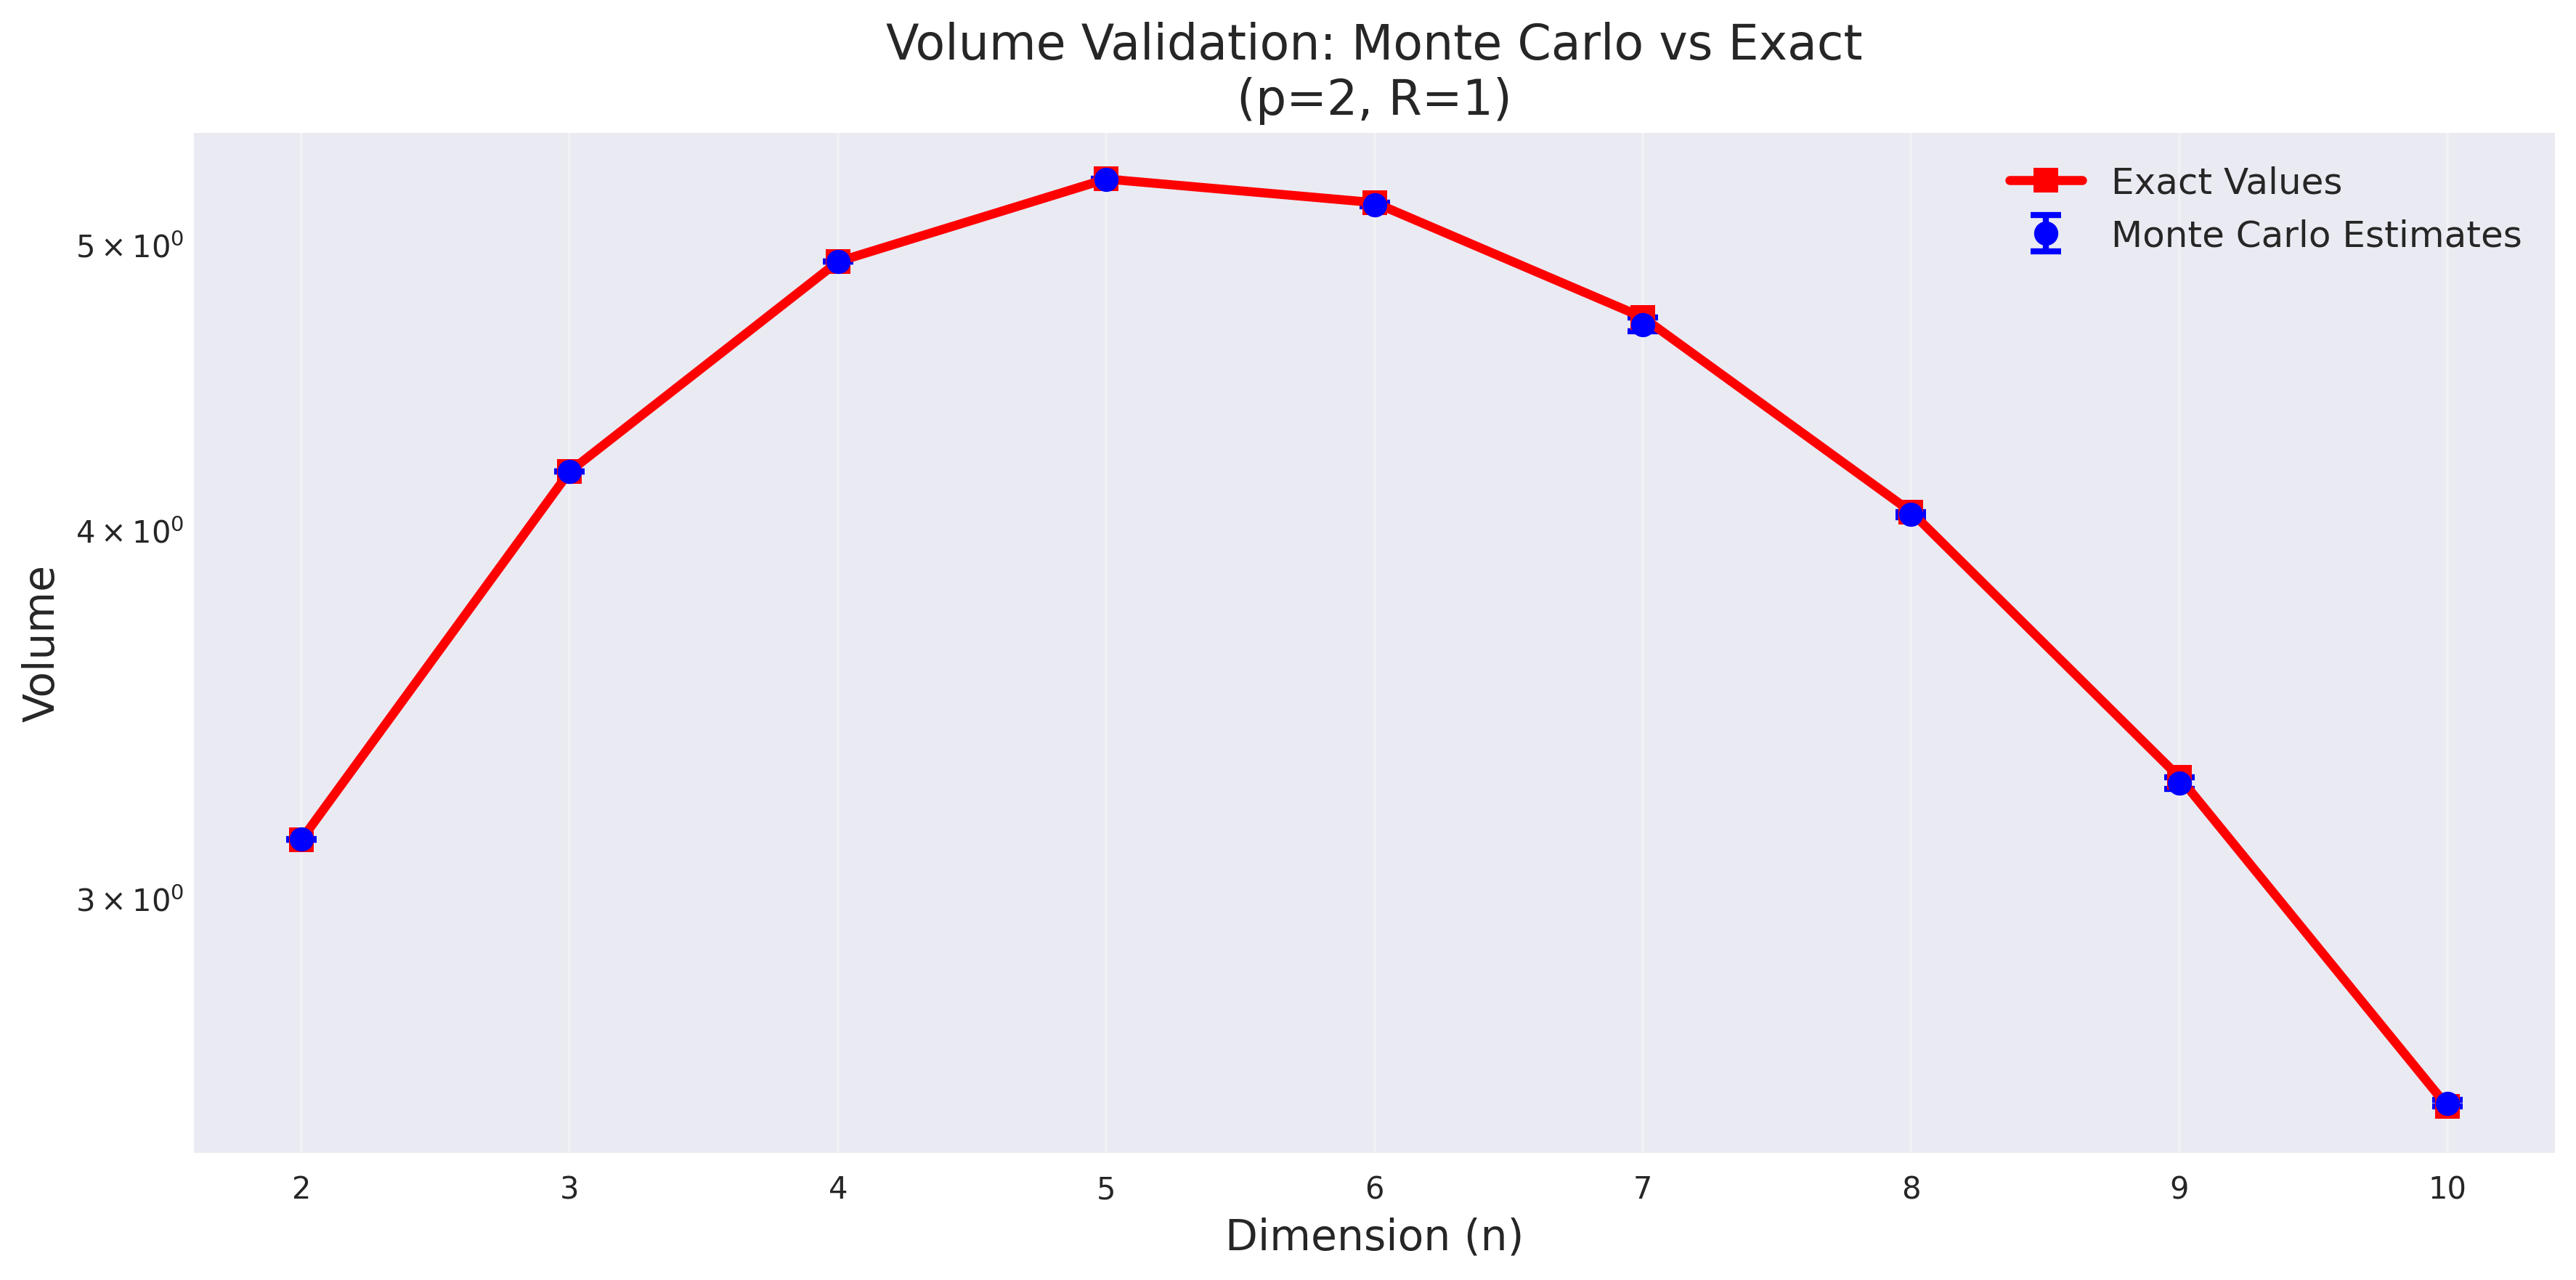
\includegraphics[width=0.9\linewidth]{../plots/validation_comparison.png}
		\caption{Validation of Monte Carlo volume estimates against exact analytical values for Euclidean spheres ($p = 2$, $R = 1$). Error bars represent estimated uncertainties based on the Monte Carlo standard error. The excellent agreement across all dimensions confirms the correctness of the implementation.}
		\label{fig:validation}
	\end{figure}
	
	The characteristic behavior of Euclidean sphere volumes is clearly visible, with volumes initially increasing with dimension (peaking around $n = 5$), then rapidly decreasing as the "curse of dimensionality" takes effect.
	
	\subsection{Accuracy Analysis}
	
	Figure~\ref{fig:accuracy} shows the relationship between Monte Carlo relative error and sample size $N$ for the test case $n = 10$, $p = 4$, $R = 1$. The results closely follow the theoretical $\mathcal{O}(1/\sqrt{N})$ scaling, as evidenced by the parallel trends between experimental data and the theoretical line.
	
	\begin{figure}[H]
		\centering
		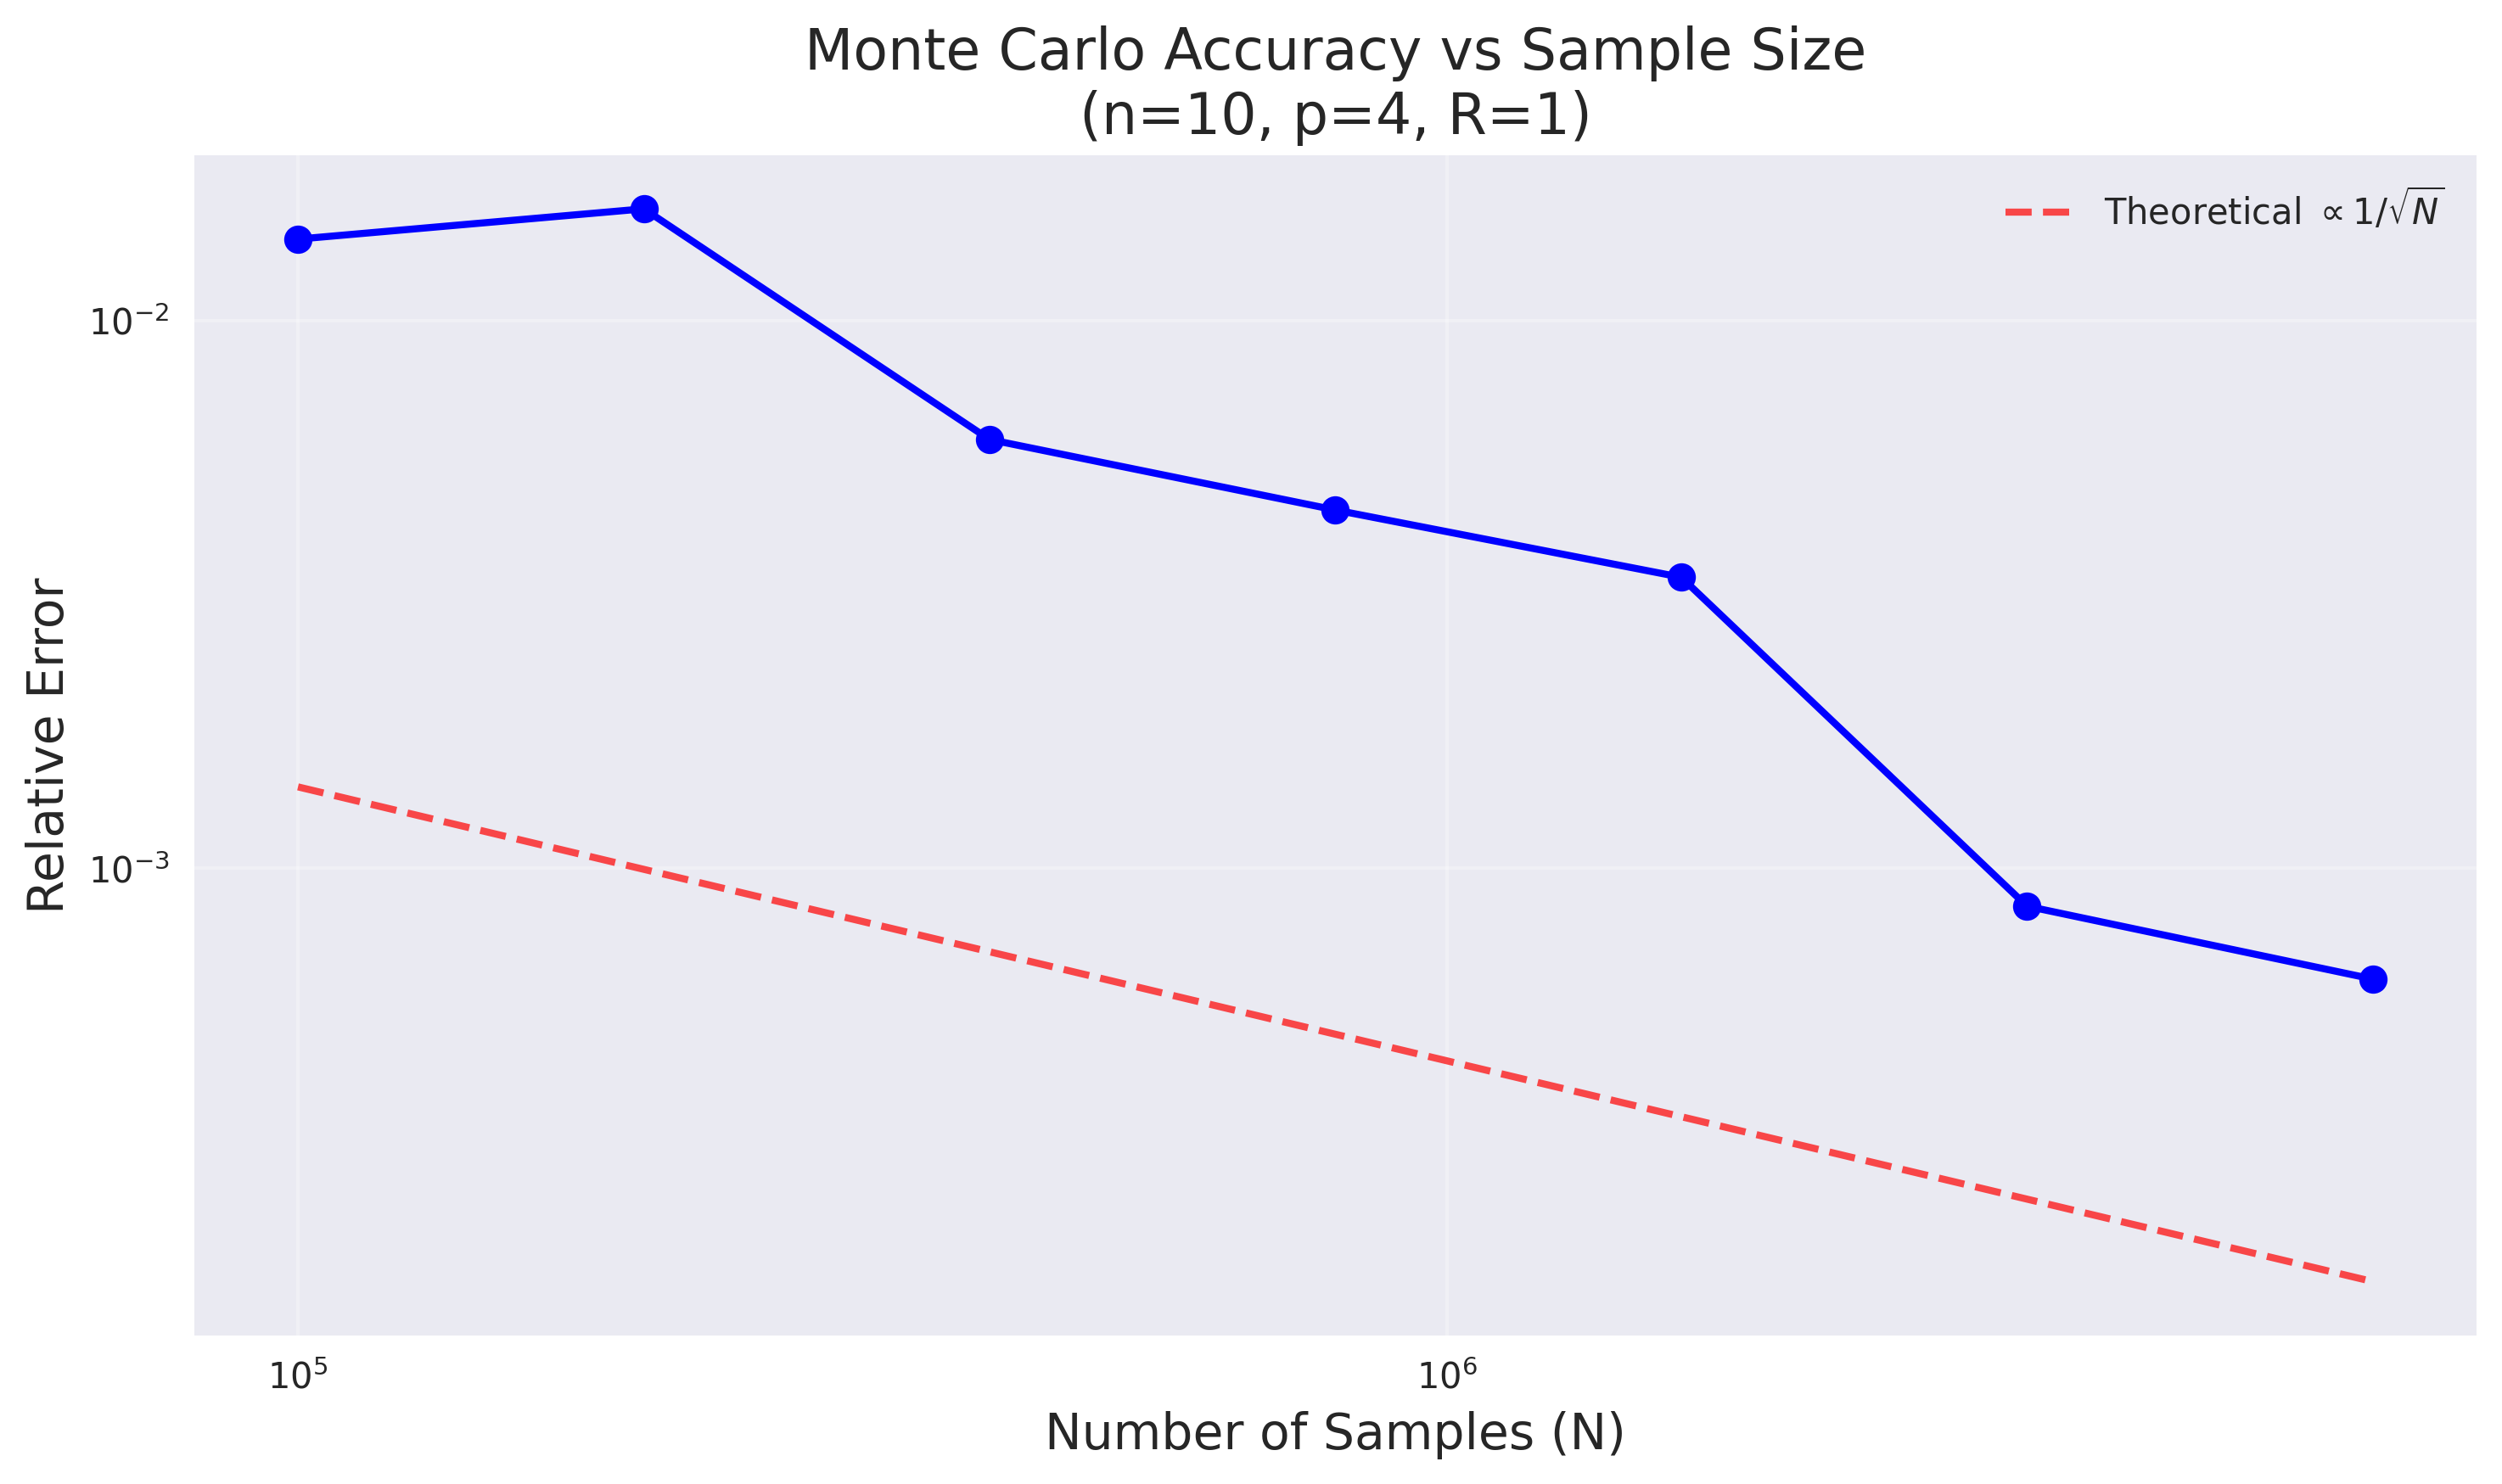
\includegraphics[width=0.9\linewidth]{../plots/accuracy_vs_n.png}
		\caption{Monte Carlo accuracy vs sample size showing the characteristic $1/\sqrt{N}$ error scaling. The experimental data (blue circles) closely follows the theoretical trend (red dashed line), confirming proper implementation. The best accuracy achieved was 0.063\% relative error with 6.4M samples.}
		\label{fig:accuracy}
	\end{figure}
	
	Key accuracy metrics are summarized in Table~\ref{table:accuracy_summary}.
	
	\begin{table}[H]
		\centering
		\caption{Accuracy analysis summary for $n=10$, $p=4$, $R=1$.}
		\label{table:accuracy_summary}
		\begin{tabular}{rrr}
			\toprule
			Sample Size ($N$) & Relative Error (\%) & Runtime (s) \\
			\midrule
			100,000 & 1.41 & 0.043 \\
			200,000 & 1.60 & 0.079 \\
			400,000 & 0.61 & 0.157 \\
			800,000 & 0.45 & 0.309 \\
			1,600,000 & 0.34 & 0.618 \\
			3,200,000 & 0.085 & 1.501 \\
			6,400,000 & 0.063 & 2.657 \\
			\bottomrule
		\end{tabular}
	\end{table}
	
	\subsection{Parallel Performance Analysis}
	
	Figure~\ref{fig:scaling} presents the parallel scaling analysis conducted with $N = 5 \times 10^6$ samples. The system achieves excellent speedup for 2 threads (2.28×) but shows performance degradation beyond this point.
	
	\begin{figure}[H]
		\centering
		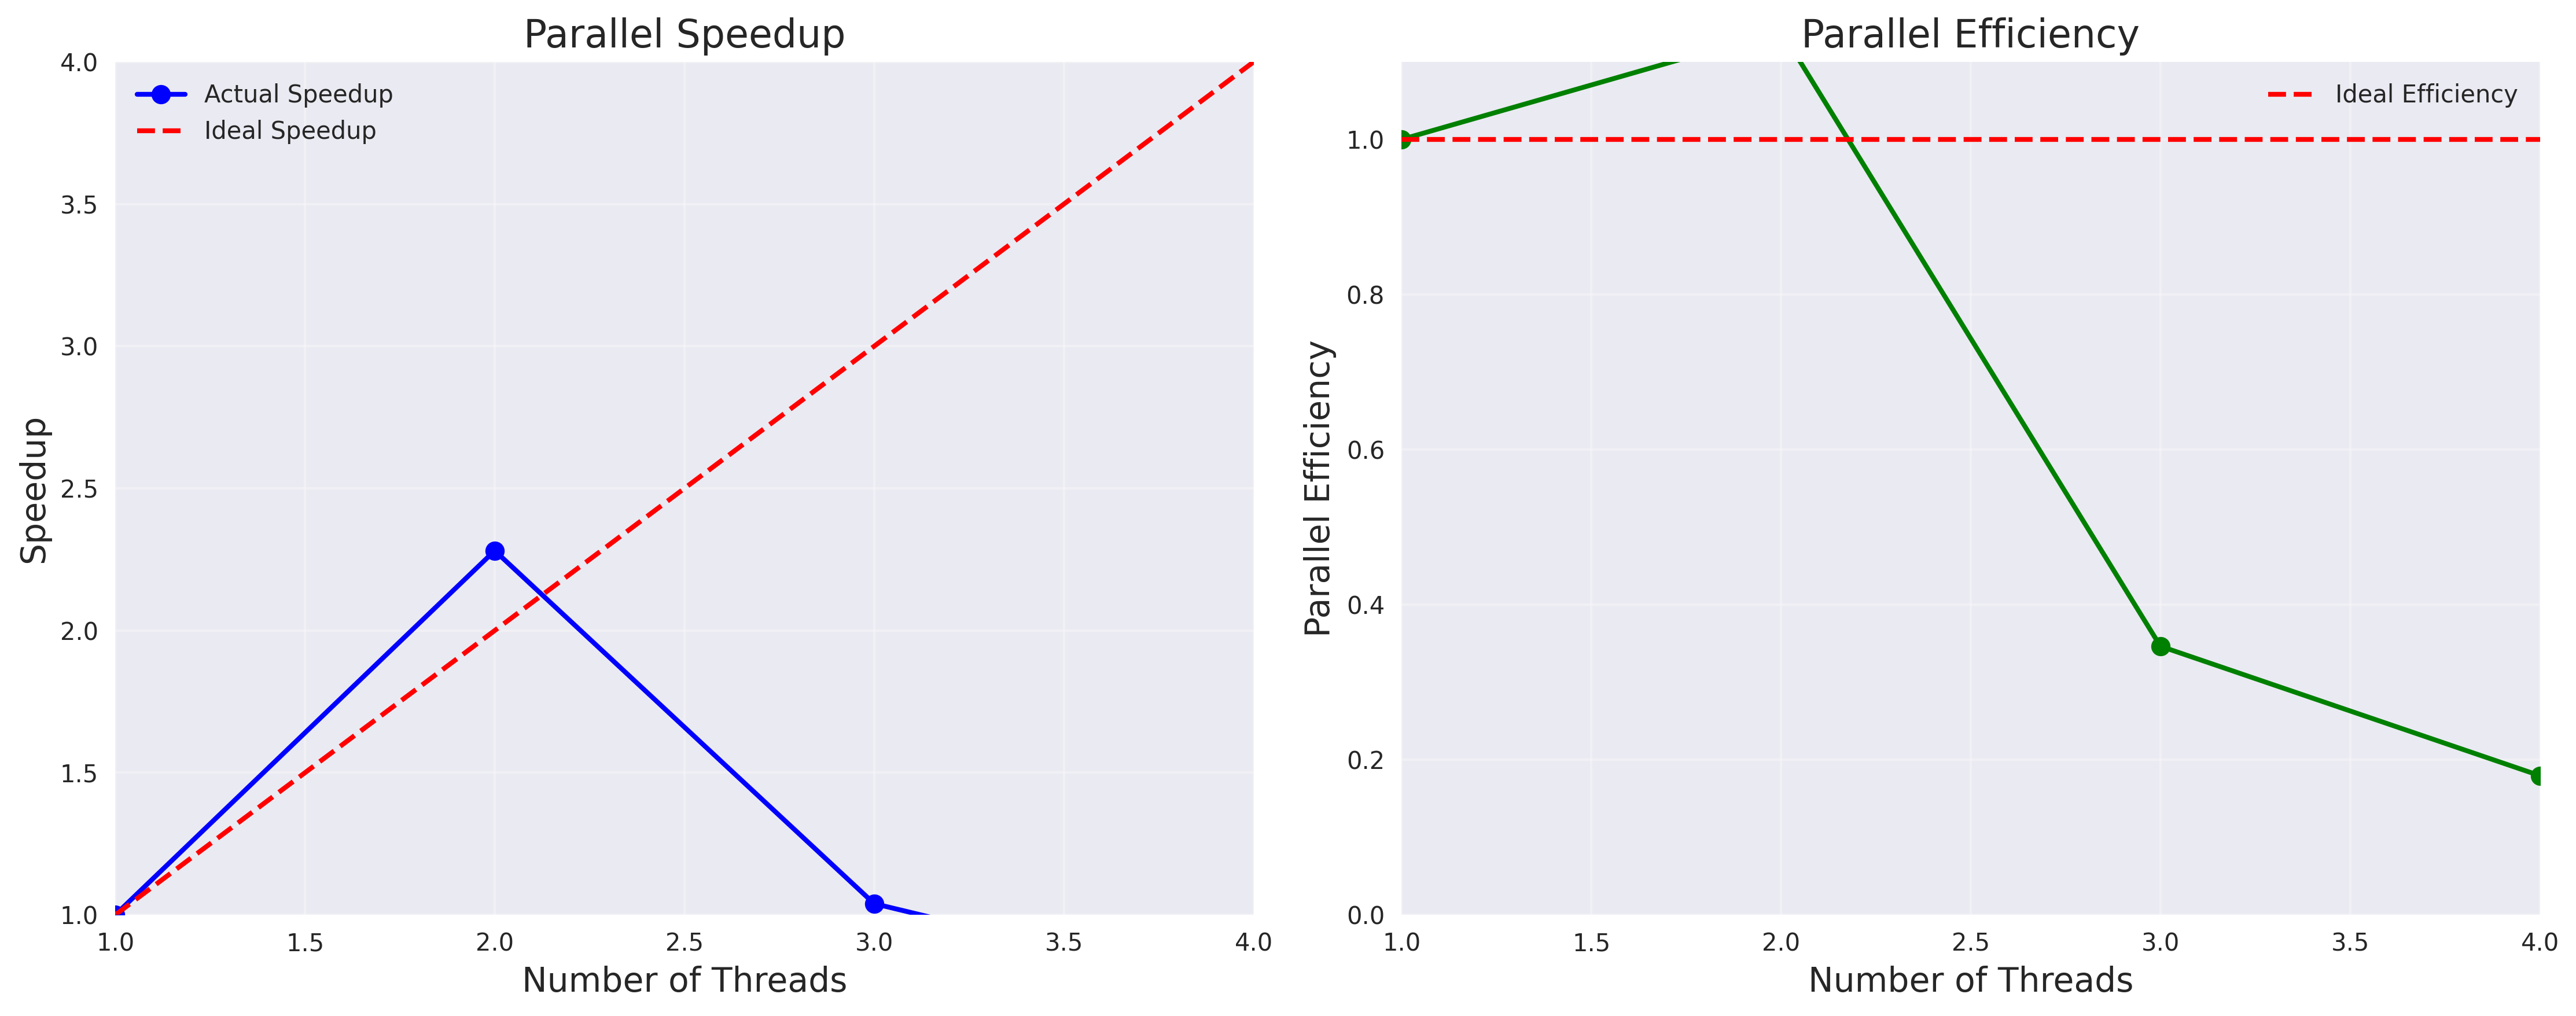
\includegraphics[width=\linewidth]{../plots/scaling_analysis.png}
		\caption{Parallel performance analysis showing (left) speedup and (right) parallel efficiency vs number of threads. The system shows good scaling up to 2 threads but degrades beyond due to hardware limitations of the dual-core system with hyperthreading.}
		\label{fig:scaling}
	\end{figure}
	
	The performance degradation beyond 2 threads is attributed to the underlying hardware architecture: the Intel i5-7200U has only 2 physical cores with hyperthreading, so threads 3-4 compete for the same physical resources, leading to reduced efficiency and increased runtime due to context switching overhead.
	
	\begin{table}[H]
		\centering
		\caption{Detailed parallel scaling results for $N = 5 \times 10^6$.}
		\label{table:scaling_results}
		\begin{tabular}{rrrrr}
			\toprule
			Threads & Runtime (s) & Speedup & Efficiency (\%) & Relative Error (\%) \\
			\midrule
			1 & 2.08 & 1.00 & 100.0 & 0.066 \\
			2 & 0.91 & 2.28 & 114.0 & 0.113 \\
			3 & 2.00 & 1.04 & 34.6 & 0.042 \\
			4 & 2.90 & 0.72 & 18.0 & 0.115 \\
			\bottomrule
		\end{tabular}
	\end{table}
	
	\subsection{OpenMP Scheduling Analysis}
	
	Figure~\ref{fig:scheduling} compares static and dynamic scheduling strategies across different chunk sizes. For this embarrassingly parallel workload with uniform computational cost per iteration, static scheduling generally provides better performance due to lower overhead.
	
	\begin{figure}[H]
		\centering
		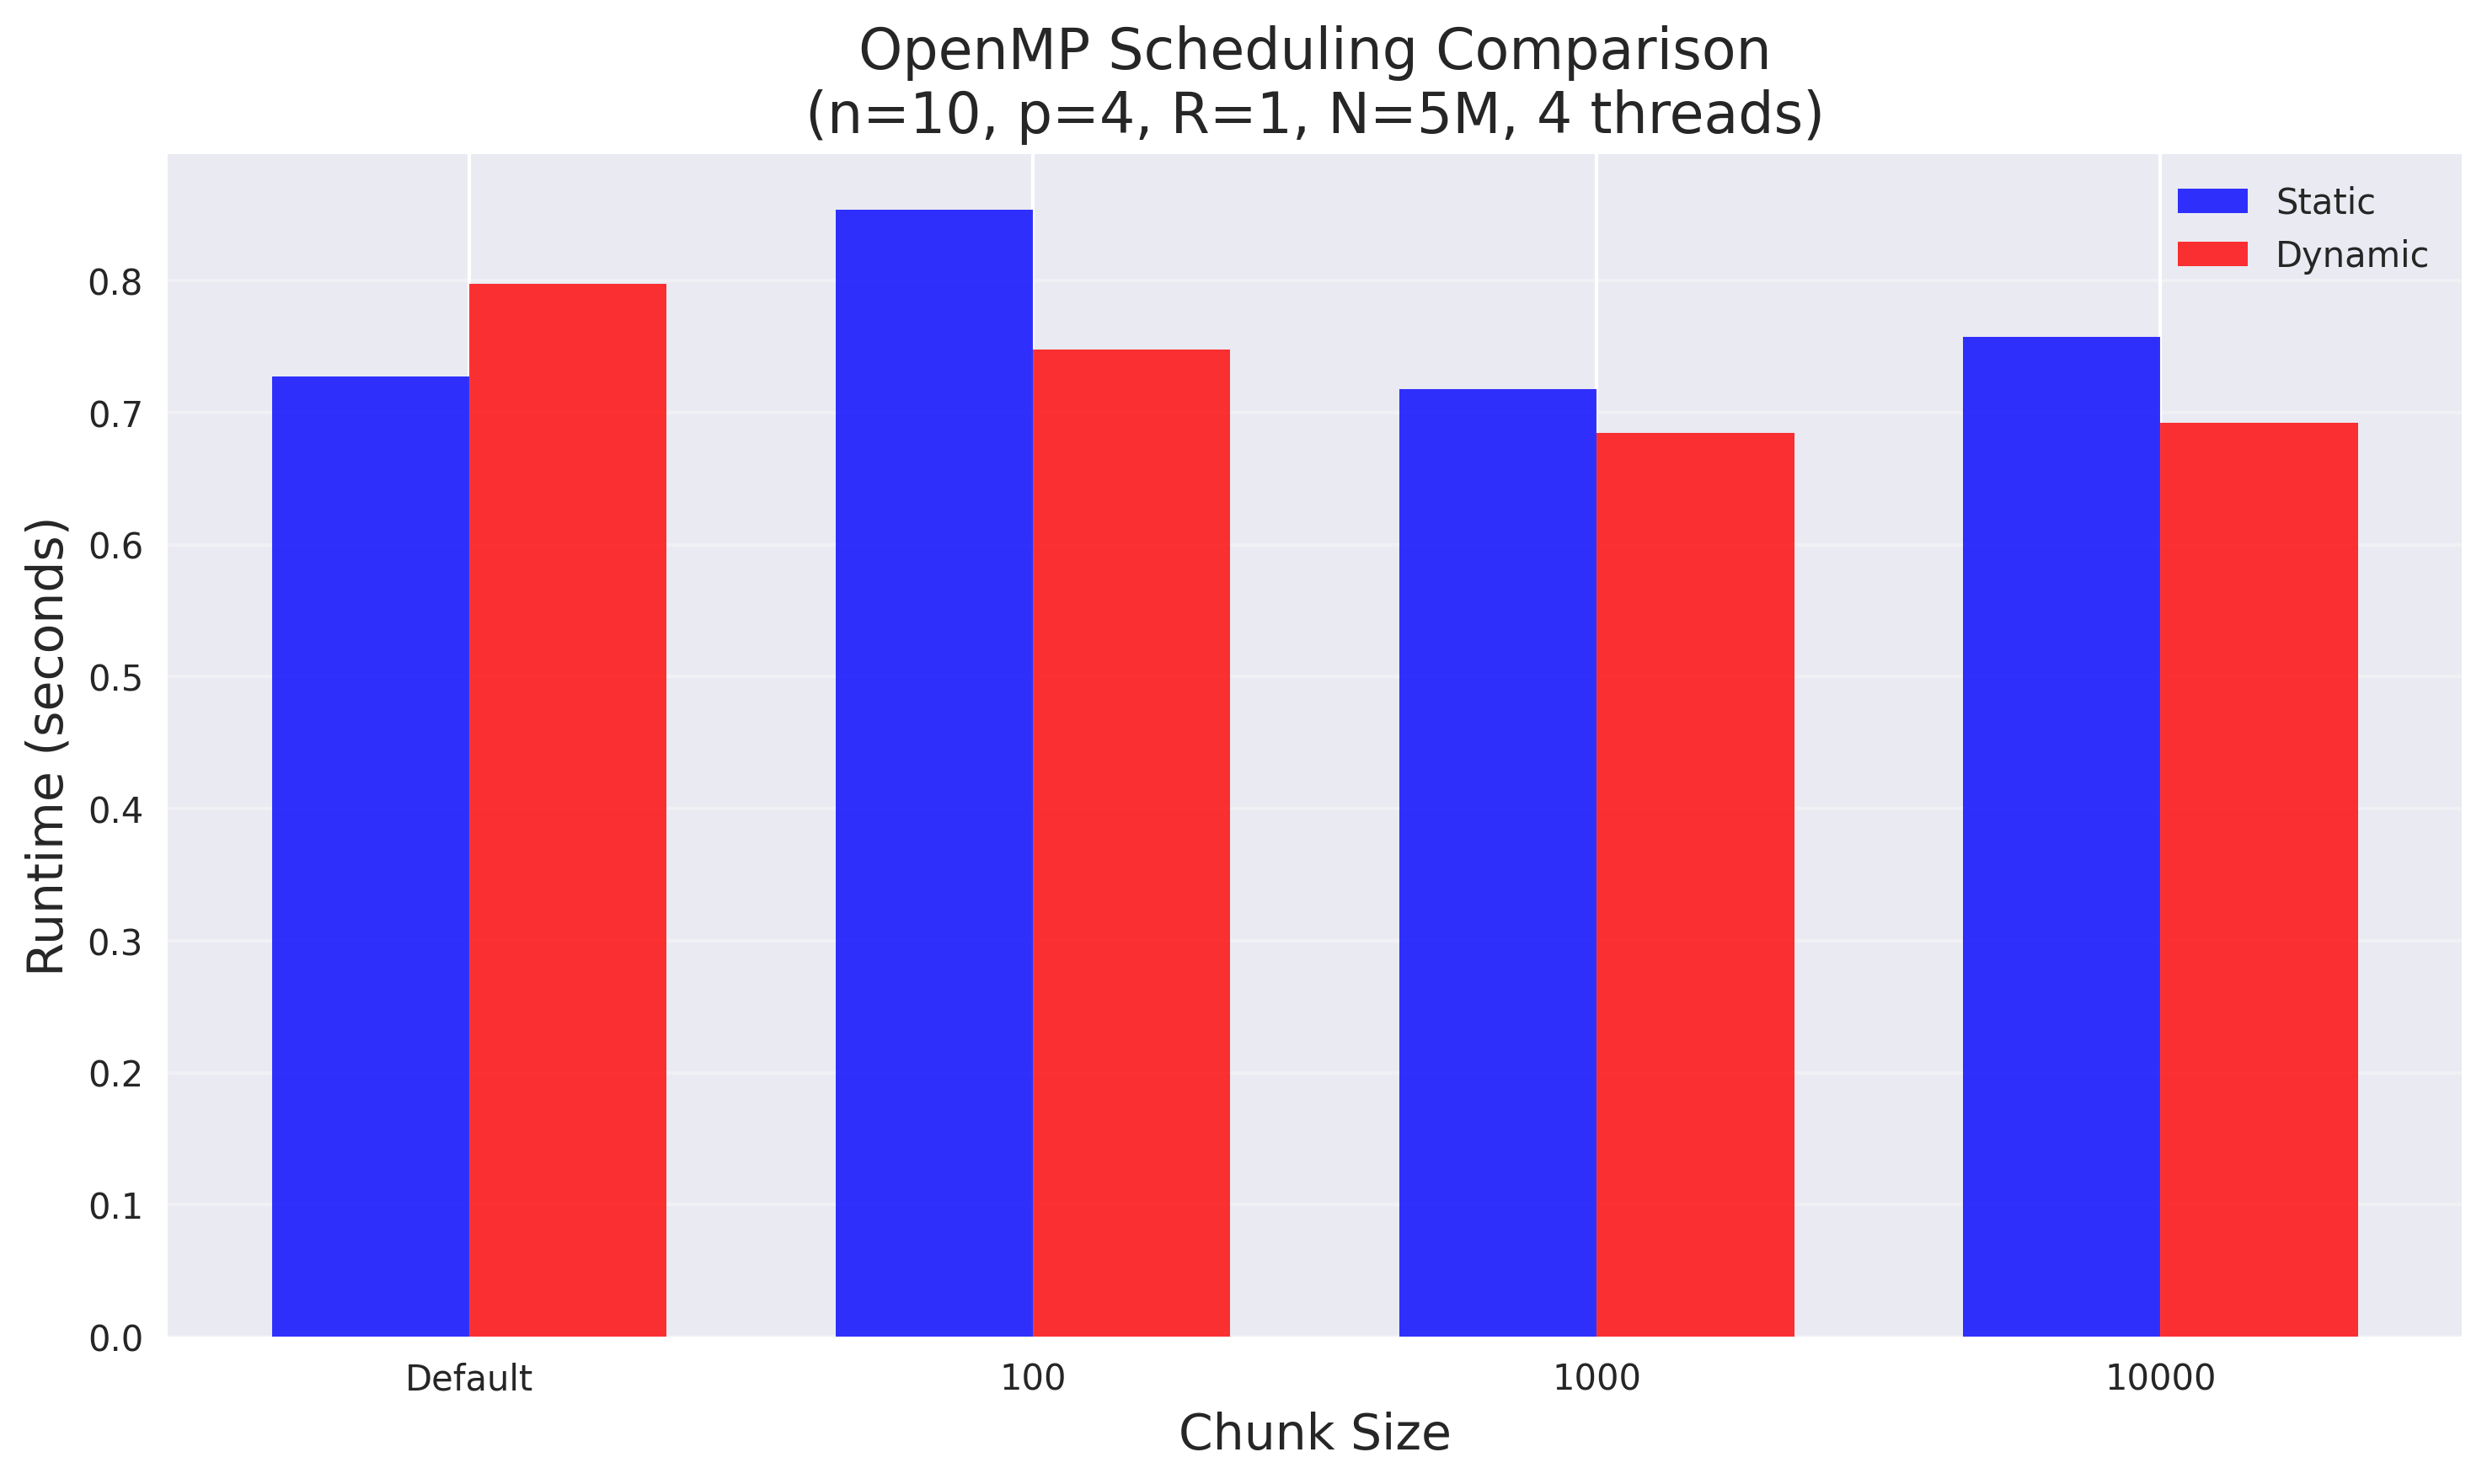
\includegraphics[width=0.9\linewidth]{../plots/schedule_comparison.png}
		\caption{Comparison of OpenMP scheduling strategies. Static scheduling generally outperforms dynamic scheduling for this uniform workload, with chunk size = 100 providing optimal performance for static scheduling.}
		\label{fig:scheduling}
	\end{figure}
	
	The results show that static scheduling with moderate chunk sizes (around 100-1000) provides the best balance between load distribution and scheduling overhead.
	
	\subsection{High-Dimensional Behavior}
	
	Figure~\ref{fig:high_dimensional} illustrates the behavior of p-spheres in higher dimensions for different values of $p$. This analysis reveals important characteristics of Monte Carlo methods in high-dimensional spaces.
	
	\begin{figure}[H]
		\centering
		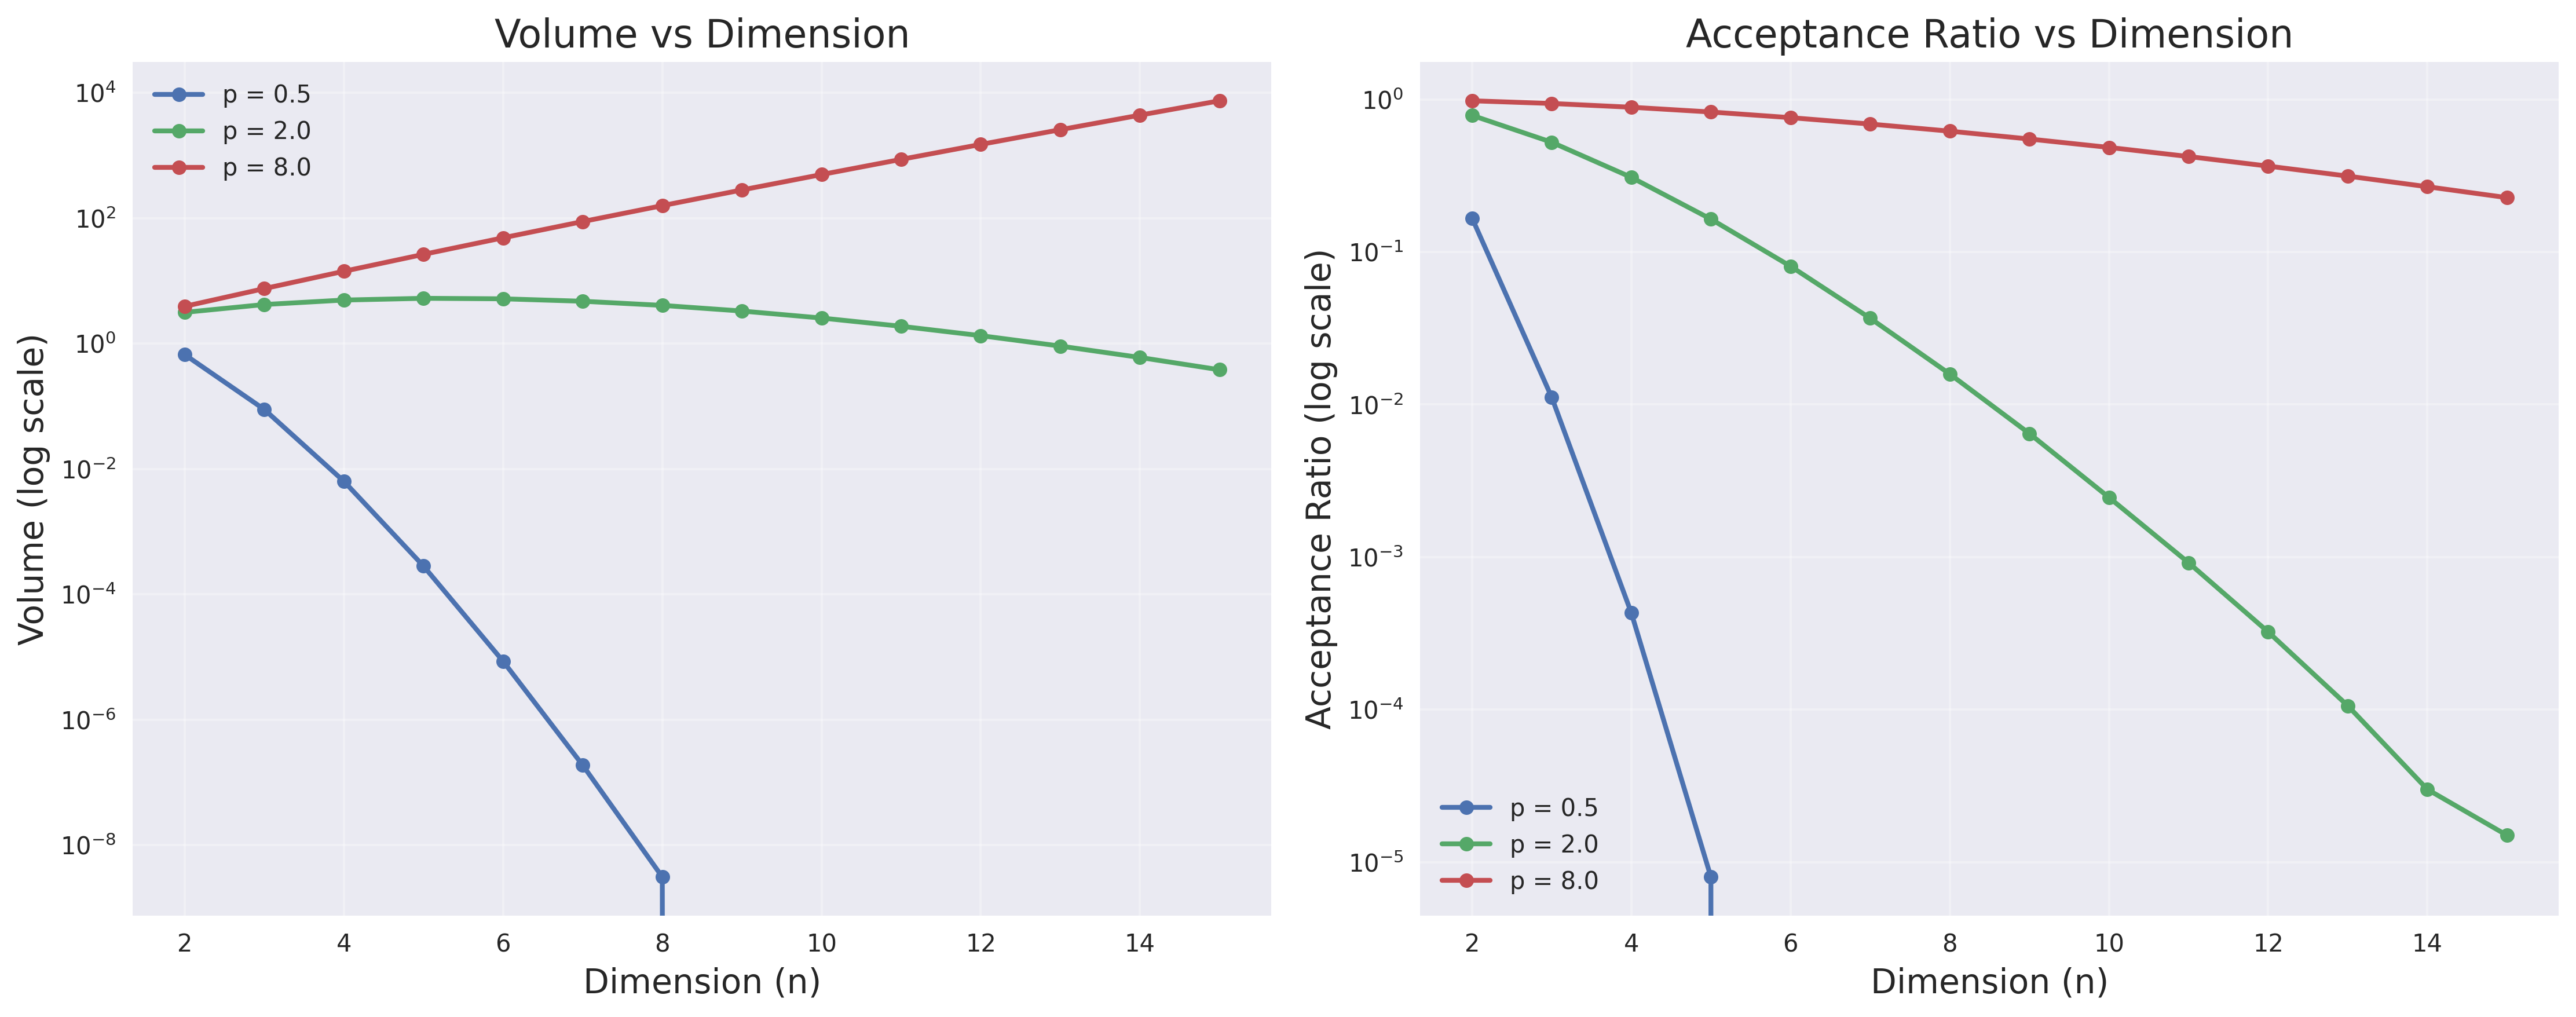
\includegraphics[width=\linewidth]{../plots/high_dimensional_behavior.png}
		\caption{High-dimensional analysis showing (left) volume vs dimension and (right) acceptance ratio vs dimension for different p-values. The rapidly decreasing acceptance ratios highlight the challenges of Monte Carlo methods in high dimensions.}
		\label{fig:high_dimensional}
	\end{figure}
	
	The acceptance ratio (fraction of samples falling within the p-sphere) decreases exponentially with dimension, particularly for $p = 0.5$ and $p = 2.0$. This demonstrates the "curse of dimensionality" where Monte Carlo methods become increasingly inefficient as the target region becomes a smaller fraction of the sampling domain.
	
	\section{Discussion}
	
	The experimental results validate both the correctness and theoretical expectations of the Monte Carlo implementation. The error scaling follows the predicted $\mathcal{O}(1/\sqrt{N})$ behavior, confirming proper statistical sampling. The parallel implementation achieves good efficiency on a dual-core system but demonstrates the importance of matching thread count to physical hardware capabilities.
	
	The scheduling analysis reveals that for uniformly distributed computational workloads, static scheduling minimizes overhead compared to dynamic scheduling. This aligns with theoretical expectations since the Monte Carlo sampling presents no load imbalancing issues.
	
	The high-dimensional analysis illustrates fundamental limitations of Monte Carlo methods as dimensionality increases. The exponentially decreasing acceptance ratios suggest that for practical high-dimensional problems, more sophisticated sampling strategies (such as importance sampling or Markov Chain Monte Carlo) would be necessary.
	
	Key bottlenecks identified include: (1) \textbf{Hardware limitations}: Performance degradation beyond physical core count due to hyperthreading overhead; (2) \textbf{Dimensional scaling}: Rapidly decreasing efficiency in high-dimensional spaces; (3) \textbf{Memory bandwidth}: Not a limiting factor for this problem size and system configuration.
	
	\section{Reproducibility}
	
	All results can be reproduced using the provided automated scripts. The complete workflow includes:
	
	1. Source code compilation with specified compiler flags
	2. Automated experiment execution with fixed random seeds (seed = 42)
	3. Data analysis and plot generation
	4. Result summarization
	
	Random seeds are fixed throughout to ensure deterministic results. The build system uses consistent compiler optimization flags (\texttt{-O3 -fopenmp}) for reproducible performance measurements.
	
	\section{Conclusion}
	
	This work successfully demonstrates the implementation and analysis of a parallel Monte Carlo method for n-dimensional sphere volume estimation. Key achievements include: (1) successful validation against analytical formulas with sub-percent accuracy; (2) demonstration of theoretical error scaling behavior; (3) effective parallelization with good efficiency on appropriate hardware; and (4) comprehensive analysis of algorithm behavior across multiple dimensions and parameters.
	
	The most impactful next steps for performance improvement would be: (1) implementation of adaptive sampling strategies for high-dimensional cases to address the curse of dimensionality; (2) investigation of vectorization techniques (SIMD) to improve single-thread performance; and (3) exploration of GPU acceleration for massively parallel sampling.
	
	\section*{Acknowledgments}
	
	The author thanks classmates for providing emotional and coding support.
	
	\section*{Honor Statement}
	\honor
	
	% No bibliography needed for this assignment
	% \printbibliography
	
	\section*{Submission Checklist}
	\begin{itemize}
		\item C source code with OpenMP parallelization
		\item Makefile with proper compilation flags
		\item \texttt{README.md} with build and run instructions
		\item Automated experiment scripts
		\item Python plotting and analysis scripts
		\item All generated data files and plots
	\end{itemize}
	
\end{document}